% select subfiles base file
\documentclass[TGAI_Laborbericht.tex]{subfiles}
\begin{document}


\chapter{Versuch 2}
\label{chap:VERSUCH_2}


\section{Fragestellung, Messprinzip, Aufbau, Messmittel}
\label{chap:VERSUCH_2_FRAGESTELLUNG}
In Versuch 2 erzeugen wir verschiedene Freqenzen und lassen diese über einen Lautsprecher von einem Mikrofon aufnehmen. Hieraus messen wir dann die Amplitude und die Phasenverschiebung. 

\subsection{Messprinzip}
Das Messprinzip entspricht dem aus Versuch 1.

\subsection{Messmittel}
Die Messmittel entsprechen auch denen aus Versuch 1.

\subsection{Aufbau}
Hier benutzen wir wieder das Oszilloskop sowie das Mikrofon aus Versuch 1. Zusätzlich haben wir nun noch einen Synthesizer und einen Lautsprecher mit dem Oszilloskop verbunden. Der Lautsprecher besitzt jeweils einen getrennten Mittel sowie einen Hochtöner.

\section{Messwerte}
\label{chap:VERSUCH_2_MESSWERTE}
Wir haben für verschiedene Frequenzen die jeweilige Amplitude und Phasenverschiebung für die entsprechenden Lautsprecher gemessen. Hierzu haben wir das Ausgangssignal mit dem Eingangssignal mithilfe des Oszilloskops verglichen. Diese Messwerte haben wir anschließend per Hand notiert und diese mithilfe eines Python skripts in numpy arrays gespeichert. 


\section{Auswertung}
\label{chap:VERSUCH_2_AUSWERTUNG}
Wir haben für jeden der beiden Lautsprecher ein Bode Diagramm erstellt. Hierzu rechnen wir den Amplitudengang in Dezibel um und stellen ihn in Abhängigkeit zur Frequenz dar. Desweiteren berechnen wir den Phasenwinkel nach der Formel \[\varphi H = -\Delta t\cdot f \cdot 360^\circ\] und stellen diesen ebenfalls in Abhängigkeit zur Frequenz dar. Die Diagramme werden jeweils halblogarithmisch dargestellt, dies geschieht mithilfe der Funktion semilogx().

\section{Interpretation}
\label{chap:VERSUCH_2_INTERPRETATION}
Wenn man den jeweiligen Phasengang der beiden Lautsprecher betrachtet sieht man dass sich der Phasenwinkel bei höherer Frequenz tendenziell verringert.
Anhand der Amplitudengänge kann man sehen, dass der große Lautsprecher eher niedrigere Frequenzen (ca. 200Hz) und der kleine Lautsprecher etwas höhere Frequenzen (ca. 500Hz) am stärksten verstärkt.

\begin{figure}[H]
	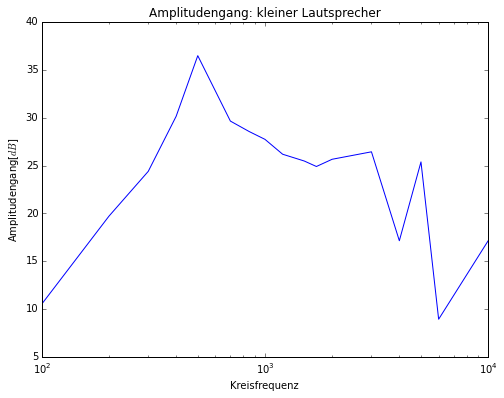
\includegraphics[width=0.7\textwidth]{media/amplitudengang_klein.png}
	\label{amplitudengang klein}
	\caption{amplitudengang klein}
\end{figure}

\begin{figure}[H]
	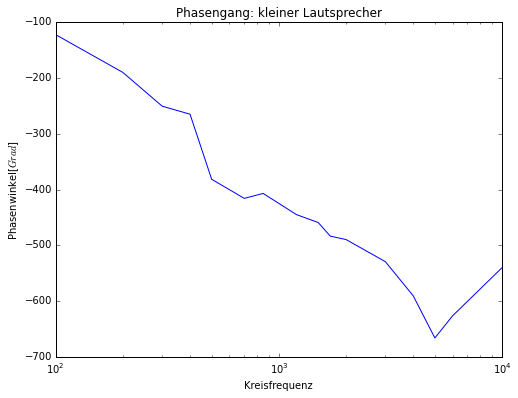
\includegraphics[width=0.7\textwidth]{media/phasengang_klein.png}
	\label{phasengang klein}
	\caption{phasengang klein}
\end{figure}

\begin{figure}[H]
	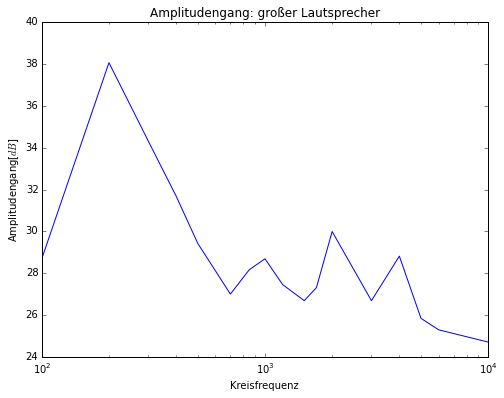
\includegraphics[width=0.7\textwidth]{media/amplitudengang_gross.png}
	\label{amplitudengang gross}
	\caption{amplitudengang gross}
\end{figure}

\begin{figure}[H]
	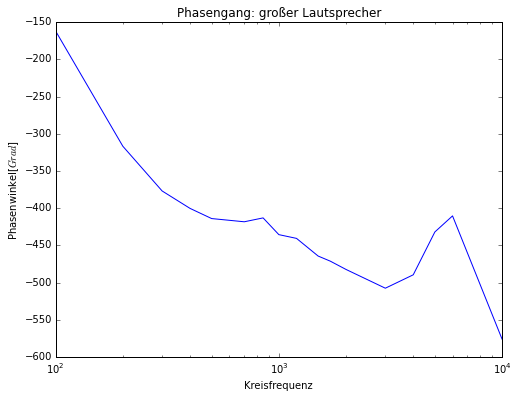
\includegraphics[width=0.7\textwidth]{media/phasengang_gross.png}
	\label{phasengang gross}
	\caption{phasengang gross}
\end{figure}

\end{document}